\break
\section{Explore the application areas of Fractal Geometry and Turing Patterns}

In applied graphics, mathematical generators like fractal recursion create scalable, efficient, and nature-inspired visual complexity.

\subsection{Fractal Geometry (Application-Focused)}
\begin{figure}[H]
\begin{minipage}{0.35\textwidth}
    \centering
    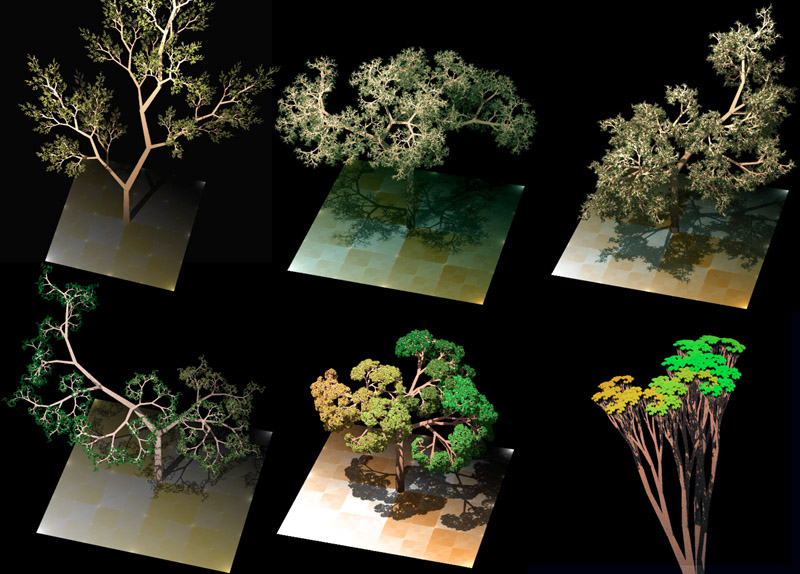
\includegraphics[width=0.5\textwidth]{img/Dragon_trees.jpg}
    \caption{L-system generated application areas}
    \label{fig:lsystem}
\end{minipage}
\hfill
\begin{minipage}{0.6\textwidth}
Fractal geometry is characterized by recursive self-similarity across scales \cite{mandelbrot1983}. In practice, it is implemented through generative systems such as \textbf{Lindenmayer systems (L-systems)} and \textbf{Iterated Function Systems (IFS)}, which allow compact rule-based generation of highly detailed forms.
\end{minipage}
\end{figure}

\textbf{Application areas:}
\begin{table}[h]
\centering
\caption{Application areas of Fractal Geometry}
\begin{tabular}{|p{4cm}|p{13cm}|}
\hline
\textbf{Application Area} & \textbf{Key Points} \\
\hline
Procedural Modeling and CGI & Terrain generation, vegetation modeling, cloud simulation. Recursive rules enable rich natural scenes with minimal memory and manual effort \cite{prusinkiewicz1990}. \\
\hline
Architectural and Generative Design & Parametric façades, structural concepts. Supports modular repetition, visual coherence, and material efficiency through fractal branching and scaling. \\
\hline
Engineering and Spatial Optimization & Antenna design, compact layout planning. Space-filling curves maximize effective path length within constrained boundaries \cite{cohen1999}. \\
\hline
\end{tabular}
\end{table}

\subsection{Turing Patterns (Application-Focused)}
Turing patterns are reaction-diffusion phenomena whose coupled differential equations generate organic, non-repetitive spatial structures for applied graphical and material design.

\textbf{Application areas:}
\begin{table}[H]
\caption{Application areas of Turing Patterns}
\centering
\begin{tabular}{|p{4cm}|p{13cm}|}
\hline
\textbf{Application Area} & \textbf{Key Points} \\
\hline
Surface and Textile Design & Biomorphic textures for textiles, product surfaces, decorative graphics. Enables variation without manual pattern design through reaction-diffusion simulations. \\
\hline
Computational Material Design & Additive manufacturing: heterogeneous material layouts, gradient stiffness, controlled deformation, functional material behavior via Turing-based distributions. \\
\hline
Motion Graphics and Visual Effects & Organic transitions, animated textures, interactive visual installations. Time-evolving systems avoid mechanical repetition. \\
\hline
\end{tabular}
\end{table}

% \begin{figure}[h]
% \centering
% \includegraphics[width=0.38\textwidth]{img/turing.png}
% \caption{Reaction--diffusion pattern illustrating spatial heterogeneity}
% \label{fig:turing}
% \end{figure}